\documentclass[11pt,a4paper,twoside]{article}
\usepackage{lmodern}
\usepackage{amssymb,amsmath}
\usepackage{ifxetex,ifluatex}
\usepackage{fixltx2e} % provides \textsubscript
\ifnum 0\ifxetex 1\fi\ifluatex 1\fi=0 % if pdftex
  \usepackage[T1]{fontenc}
  \usepackage[utf8]{inputenc}
\else % if luatex or xelatex
  \ifxetex
    \usepackage{mathspec}
  \else
    \usepackage{fontspec}
  \fi
  \defaultfontfeatures{Ligatures=TeX,Scale=MatchLowercase}
\fi
% use upquote if available, for straight quotes in verbatim environments
\IfFileExists{upquote.sty}{\usepackage{upquote}}{}
% use microtype if available
\IfFileExists{microtype.sty}{%
\usepackage{microtype}
\UseMicrotypeSet[protrusion]{basicmath} % disable protrusion for tt fonts
}{}
\usepackage[left=2.5cm,right=3.5cm,top=83.75pt,textheight=24.35cm,textwidth=15cm,a4paper,headheight=13.6pt,twoside=true]{geometry}
\usepackage{hyperref}
\hypersetup{unicode=true,
            pdfborder={0 0 0},
            breaklinks=true}
\urlstyle{same}  % don't use monospace font for urls
\usepackage{biblatex}

\addbibresource{bibliography.bib}
\addbibresource{packages.bib}
\usepackage{longtable,booktabs}
\usepackage{graphicx,grffile}
\makeatletter
\def\maxwidth{\ifdim\Gin@nat@width>\linewidth\linewidth\else\Gin@nat@width\fi}
\def\maxheight{\ifdim\Gin@nat@height>\textheight\textheight\else\Gin@nat@height\fi}
\makeatother
% Scale images if necessary, so that they will not overflow the page
% margins by default, and it is still possible to overwrite the defaults
% using explicit options in \includegraphics[width, height, ...]{}
\setkeys{Gin}{width=\maxwidth,height=\maxheight,keepaspectratio}
\IfFileExists{parskip.sty}{%
\usepackage{parskip}
}{% else
\setlength{\parindent}{0pt}
\setlength{\parskip}{6pt plus 2pt minus 1pt}
}
\setlength{\emergencystretch}{3em}  % prevent overfull lines
\providecommand{\tightlist}{%
  \setlength{\itemsep}{0pt}\setlength{\parskip}{0pt}}
\setcounter{secnumdepth}{5}

%%% Use protect on footnotes to avoid problems with footnotes in titles
\let\rmarkdownfootnote\footnote%
\def\footnote{\protect\rmarkdownfootnote}

%%% Change title format to be more compact
\usepackage{titling}

% Create subtitle command for use in maketitle
\newcommand{\subtitle}[1]{
  \posttitle{
    \begin{center}\large#1\end{center}
    }
}

\setlength{\droptitle}{-2em}

  \title{}
    \pretitle{\vspace{\droptitle}}
  \posttitle{}
    \author{}
    \preauthor{}\postauthor{}
    \date{}
    \predate{}\postdate{}
  
\usepackage{booktabs}
\usepackage[ngerman,english]{babel} % deutsche Trennregeln, "Inhaltsverzeichnis" etc.
\usepackage{mathptmx} % Times-Roman-Schrift (auch für mathematische Formeln)
\usepackage{pdfpages}
\usepackage{pgf}
\usepackage{epstopdf}

\usepackage[labelfont=bf]{caption}
\usepackage{changepage}
\usepackage{subcaption}
\usepackage{hanging}

% custom imports
% multirows für Tabellen
\usepackage{multirow}
% nice quotes
\usepackage[autostyle=true,german=quotes]{csquotes}

\usepackage[onehalfspacing]{setspace} % 1,5facher Zeilenabstand

% Zum Setzen von URLs
\usepackage{color}
\definecolor{darkred}{rgb}{0.25,0,0}
\definecolor{darkgreen}{rgb}{0,0.2,0}
\definecolor{darkmagenta}{rgb}{0.2,0,0.2}
\definecolor{darkcyan}{rgb}{0,0.15,0.15}

\usepackage{fancyhdr} % Positionierung der Seitenzahlen

\renewcommand{\headrulewidth}{0pt}

% Korrektes Format für Nummerierung von Abbildungen (figure) und
% Tabellen (table): <Kapitelnummer>.<Abbildungsnummer>
\makeatletter
\@addtoreset{figure}{section}
\renewcommand{\thefigure}{\thesection.\arabic{figure}}
\@addtoreset{table}{section}
\renewcommand{\thetable}{\thesection.\arabic{table}}
\makeatother

% include bibliography in ToC - special case for biblatex (bookdown doesn't handle this atm)
\let\oldpb\printbibliography
\renewcommand{\printbibliography}{\oldpb[heading=bibintoc]}

\let\oldpar\paragraph
\renewcommand{\paragraph}{\oldpar*}

\let\oldsubpar\subparagraph
\renewcommand{\subparagraph}{\oldsubpar*}

%\sloppy % Damit LaTeX nicht so viel über "overfull hbox" u.Ä. meckert

% römische numerale für Inhaltsverzeichnis; wird in index.Rmd zurückgesetzt
\fancyhead[LE,RO,LO,RE]{}
\fancyfoot[CE,CO,RE,LO]{}
\fancyfoot[LE,RO]{\roman{page}}

\begin{document}

\pagestyle{empty} % Vorerst keine Seitenzahlen
\pagenumbering{alph} % Unsichtbare alphabetische Nummerierung

\begin{center}
\textsc{Ludwig-Maximilians-Universität München}\\
Department ``Institut für Informatik''\\
Professur für Computational Social Science and Big Data\\
Prof.\ Jürgen Pfeffer

\vspace{4.75cm}
{\large\textbf{Masterarbeit}}\vspace{.5cm}

{\Huge{}Not all those who wander are lost}\\\vspace{.5cm}
{\Large{}Dynamiken bei der Interessensentwicklung in Online Communities}\vspace{.75cm}

{\large Oliver Baumann}\\\href{mailto:baumanno@cip.ifi.lmu.de}{<baumanno@cip.ifi.lmu.de>}

\end{center}
\vfill

\begin{tabular}{ll}
Bearbeitungszeitraum: & 30.04.2018 bis 29.10.2018\\
Betreuer: & Dr.\ Mirco Schönfeld\\
Verantw. Hochschullehrer: & Prof.\ Jürgen Pfeffer
\end{tabular}

%______________________________________________________________________

\clearpage
\section*{Zusammenfassung}

Die vorliegende Arbeit reiht sich in Forschungsliteratur zu interaktiven Tischen, interaktiven Arbeitsumgebungen,
gekrümmten Multitouch-Displays und indirekten Multitouch-Mappings ein. Anhand einer Nutzerstudie wird die Wirkung zweier indirekter
Eingabemodi auf den Nutzer untersucht. Dazu wurde für \emph{Curve}, ein interaktiver Tisch mit gebogenem Display,
eine prototypische Anwendung entwickelt, die entweder mit einer Maus oder über Multitouch-Gesten bedient werden kann.
Im Gegensatz zu isolierten Tasks ermöglicht die Anwendung den von einer Desktopumgebung gewohnten Arbeitsablauf. Das System
bietet für den Anwendungsfall "`Audio-Bearbeitung"' die Möglichkeit, in einem Audio-Sample zu navigieren und dieses
zu modifizieren. Die beiden Interface-Varianten wurden auf ihre Wirkung auf das Nutzererlebnis und ihre Eignung
zum Einsatz in interaktiven Arbeitsplätzen hin untersucht. Es wurde festgestellt, dass keine der beiden Varianten
dabei übermäßig gut oder schlecht abschneidet. Beide Eingabetechniken sind dabei ähnlich gut für den speziellen
Anwendungsfall geeignet. Ein Transfer zu anderen Einsatzmöglichkeiten schließt die Arbeit ab. Es sei darauf hingewiesen,
dass die in dieser Studie präsentierten Ergebnisse anhand einer kleinen Stichprobe ermittelt wurden und möglicherweise
nicht vollends generalisierbar sind.

\iffalse
\selectlanguage{english}
\section*{Abstract}

We relate in parts to previous work on interactive desks, interactive workspaces, bent multitouch-enabled displays
and indirect mappings for multitouch. Based on a user-study, we compare the effects of two interaction techniques on the user.
To this end, we implemented a prototypical application for \emph{Curve}, an interactive desk with a bent multitouch-display.
The user can interact with the application either via a mouse, or via multitouch-gestures.
In contrast to isolated tasks commonly used, our system enables a workflow comparable to that of a traditional desktop
environment. The system relates to the specific use-case of audio-editing and allows for navigating and manipulating an audio-sample.
Both interaction techniques presented here have been studied with regard to their effect on user experience and their
compatibility with being used in interactive workspaces. We conclude that neither of the two techniques out- or underperforms
and thus suggest that they are equally suitable for this particular use case. We end with suggesting other possible applications
of this setup, not restricted to any single use-case. We note, however, that due to the small sample size of our study, the
findings presented here might not be fully generalizable.
\selectlanguage{ngerman}
\fi
\clearpage
\section*{Eidesstattliche Erklärung}

\selectlanguage{ngerman}

\noindent Ich erkläre hiermit, dass ich die vorliegende Arbeit
selbstständig angefertigt, alle Zitate als solche kenntlich gemacht
sowie alle benutzten Quellen und Hilfsmittel angegeben habe.

\vspace{7ex}
\noindent\makebox[9.3cm]{\dotfill}

\smallskip\noindent München, \today

%______________________________________________________________________

\cleardoublepage

\pagestyle{fancy}
\pagenumbering{roman} % Römische Seitenzahlen
\setcounter{page}{1}

{
\setcounter{tocdepth}{3}
\tableofcontents
}
\cleardoublepage

\pagenumbering{arabic}
\setcounter{page}{1}

\fancyhead[LE,RO]{\rightmark}
\fancyhead[LO,RE]{\leftmark}
\fancyfoot[LE,RO]{\thepage}

\cleardoublepage

\hypertarget{einleitung}{%
\section{Einleitung}\label{einleitung}}

\cleardoublepage

\hypertarget{grundlagen-und-verwandte-forschung}{%
\section{Grundlagen und verwandte
Forschung}\label{grundlagen-und-verwandte-forschung}}

\hypertarget{topic-modelle}{%
\subsection{Topic-Modelle}\label{topic-modelle}}

\hypertarget{lda}{%
\subsubsection{LDA}\label{lda}}

\hypertarget{verwandte-arbeiten}{%
\subsubsection{Verwandte Arbeiten}\label{verwandte-arbeiten}}

\hypertarget{soziale-netzwerkanalyse}{%
\subsection{Soziale Netzwerkanalyse}\label{soziale-netzwerkanalyse}}

\hypertarget{graphen-und-netzwerke}{%
\subsubsection{Graphen und Netzwerke}\label{graphen-und-netzwerke}}

\hypertarget{ego-netzwerke}{%
\subsubsection{Ego-Netzwerke}\label{ego-netzwerke}}

\hypertarget{verwandte-arbeiten-1}{%
\subsubsection{Verwandte Arbeiten}\label{verwandte-arbeiten-1}}

\hypertarget{reddit}{%
\subsection{Reddit}\label{reddit}}

\hypertarget{begriffsklarung}{%
\subsubsection{Begriffsklärung}\label{begriffsklarung}}

\hypertarget{verwandte-arbeiten-2}{%
\subsubsection{Verwandte Arbeiten}\label{verwandte-arbeiten-2}}

\cleardoublepage

\hypertarget{datenanalyse}{%
\section{Datenanalyse}\label{datenanalyse}}

Dieses Kapitel liefert einen Überblick über die Methodik sowie die
Ergebnisse der Datenanalyse. Zunächst wird der verwendete Datensatz
präsentiert und Kritik daran erörtert. Weiterhin wird dargelegt, wie die
betrachteten Topic-Modelle erzeugt werden und welche Methoden der
sozialen Netzwerkanalyse Anwendung finden, sowie welche
Software-Komponenten jeweils zum Einsatz kommen. Im zweiten Teil des
Kapitels werden dann die Ergebnisse vorgestellt, ohne dabei jedoch einer
Interpretation zu weit vorzugreifen.

\hypertarget{methodik}{%
\subsection{Methodik}\label{methodik}}

\hypertarget{datensatz}{%
\subsubsection{Datensatz}\label{datensatz}}

Die Grundlage der Analyse bildet ein frei zugänglicher Datensatz mit
Reddit-Kommentaren. Jason Baumgartner, der unter dem Pseudonym
\emph{stuck\_in\_the\_matrix}\footnote{\url{https://www.reddit.com/user/stuck_in_the_matrix}}
selbst auf Reddit aktiv ist, stellt monatliche Zusammenfassungen aller
erstellten Kommentare zum Download bereit \autocite{Baumgartner}. Diese
reichen zum gegenwärtigen Zeitpunkt von Oktober 2018 zurück bis Dezember
2005.

\hypertarget{struktur}{%
\paragraph{Struktur}\label{struktur}}

Die monatlichen Datensätze liegen in Form von Textdateien vor, in denen
jede Zeile einen Kommentar sowie Metadaten enthält. Das maschinenlesbare
JSON-Format, in dem die Daten abgelegt sind, ermöglicht dabei eine
effiziente computergestützte Auswertung. Tabelle \ref{tab:importantkeys}
führt die für diese Arbeit relevanten Schlüssel-Wert-Paare des
Datensatzes auf. Der Schlüssel \emph{parent\_id} bezeichnet dabei das
Element, auf welches sich der Kommentar bezieht. Dies können Beiträge
oberster Ordnung sein, sog. \enquote{Links}, oder selbst Kommentare
\autocite{Reddit2018}. Zu beachten ist hier insbesondere, dass der
eigentliche Textinhalt des Kommentars für diese Auswertung nicht genutzt
wird.

\begin{table}

\caption{\label{tab:importantkeys}wichtige Schlüssel-Wert-Paare des Datensatzes}
\centering
\begin{tabular}[t]{ll}
\toprule
Schlüssel & Wert\\
\midrule
author & Username des Kommentar-Erstellers\\
id & eindeutige ID des Kommentars\\
parent\_id & eindeutige ID des Elements, auf das sich der Kommentar bezieht\\
subreddit & Name des Subreddits, in dem der Kommentar erstellt wurde\\
\bottomrule
\end{tabular}
\end{table}

\hypertarget{koharenz-des-datensatzes}{%
\paragraph{Kohärenz des Datensatzes}\label{koharenz-des-datensatzes}}

Im März 2018 haben Gaffney und Matias eine Analyse des
Baumgartner-Korpus vorgelegt \autocite{Gaffney2018}. Der vollständige
Korpus enthält neben Kommentaren auch Datensätze mit allen monatlich
erstellten Beiträgen, im folgenden auch \enquote{Submissions} genannt.
Gaffney und Matias kommen zu dem Schluss, dass die Erfassung sowohl der
Submissions als auch der Kommentare Lücken aufweist, also Elemente
gänzlich nicht im Datensatz vorhanden sind. Für den Gegenstand der
vorliegenden Arbeit ist dieser Umstand insofern von Bedeutung, als dass
fehlende Kommentare die Topic-Affinität von Nutzern verzerren können,
etwa wenn ein Topic, in dem der Nutzer durchaus aktiv war, aufgrund
fehlender Daten unterrepräsentiert ist. Auch Gaffney und Matias stellen
fest, dass Studien, welche auf die vollständige Historie von Nutzern
zugreifen, dem höchsten Risiko ausgesetzt sind, lückenhafte Daten zu
betrachten \autocite{Gaffney2018}.

Reddit weist jedem Kommentar eine eindeutige numerische ID zu. Das von
Baumgartner eingesetzte System nimmt zusammenhängende Blöcke von jeweils
100 solcher IDs und versucht, die zugehörigen Kommentare über die
Reddit-API\footnote{\url{https://api.reddit.com/}} aufzulösen
\autocite{Baumgartner2018a}. Da Reddit auch Anfragen nach gelöschten
Elementen sinnvoll beantwortet, also nicht etwa mit einer Fehlermeldung,
sollte ein Bereich von 100 sequentiellen IDs auch vollständig im
Datensatz abgebildet sein, inklusive als gelöscht markierter Elemente.
Gaffney und Matias stellen jedoch für den Zeitraum Dezember 2005 bis
Februar 2016 fest, dass 943.755 Kommentar- und 1.539.583 Beitrags-IDs
nicht in den Datensätzen enthalten sind. Als mögliche Gründe für das
Fehlen nennen Gaffney und Matias dreierlei: sog. \enquote{dangling
references}, also Verweise, bei denen das Element, auf das verwiesen
wird, nicht auffindbar ist; öffentlich zugängliche Daten, die aus
unbekanntem Grund nicht von Reddit an Baumgartners System übertragen
wurden; oder Daten aus als privat eingestuften Communities, die nicht
öffentlich sondern nur von Mitgliedern mit Zugangsberechtigung einsehbar
sind \autocite{Gaffney2018}.







\begin{figure}

{\centering 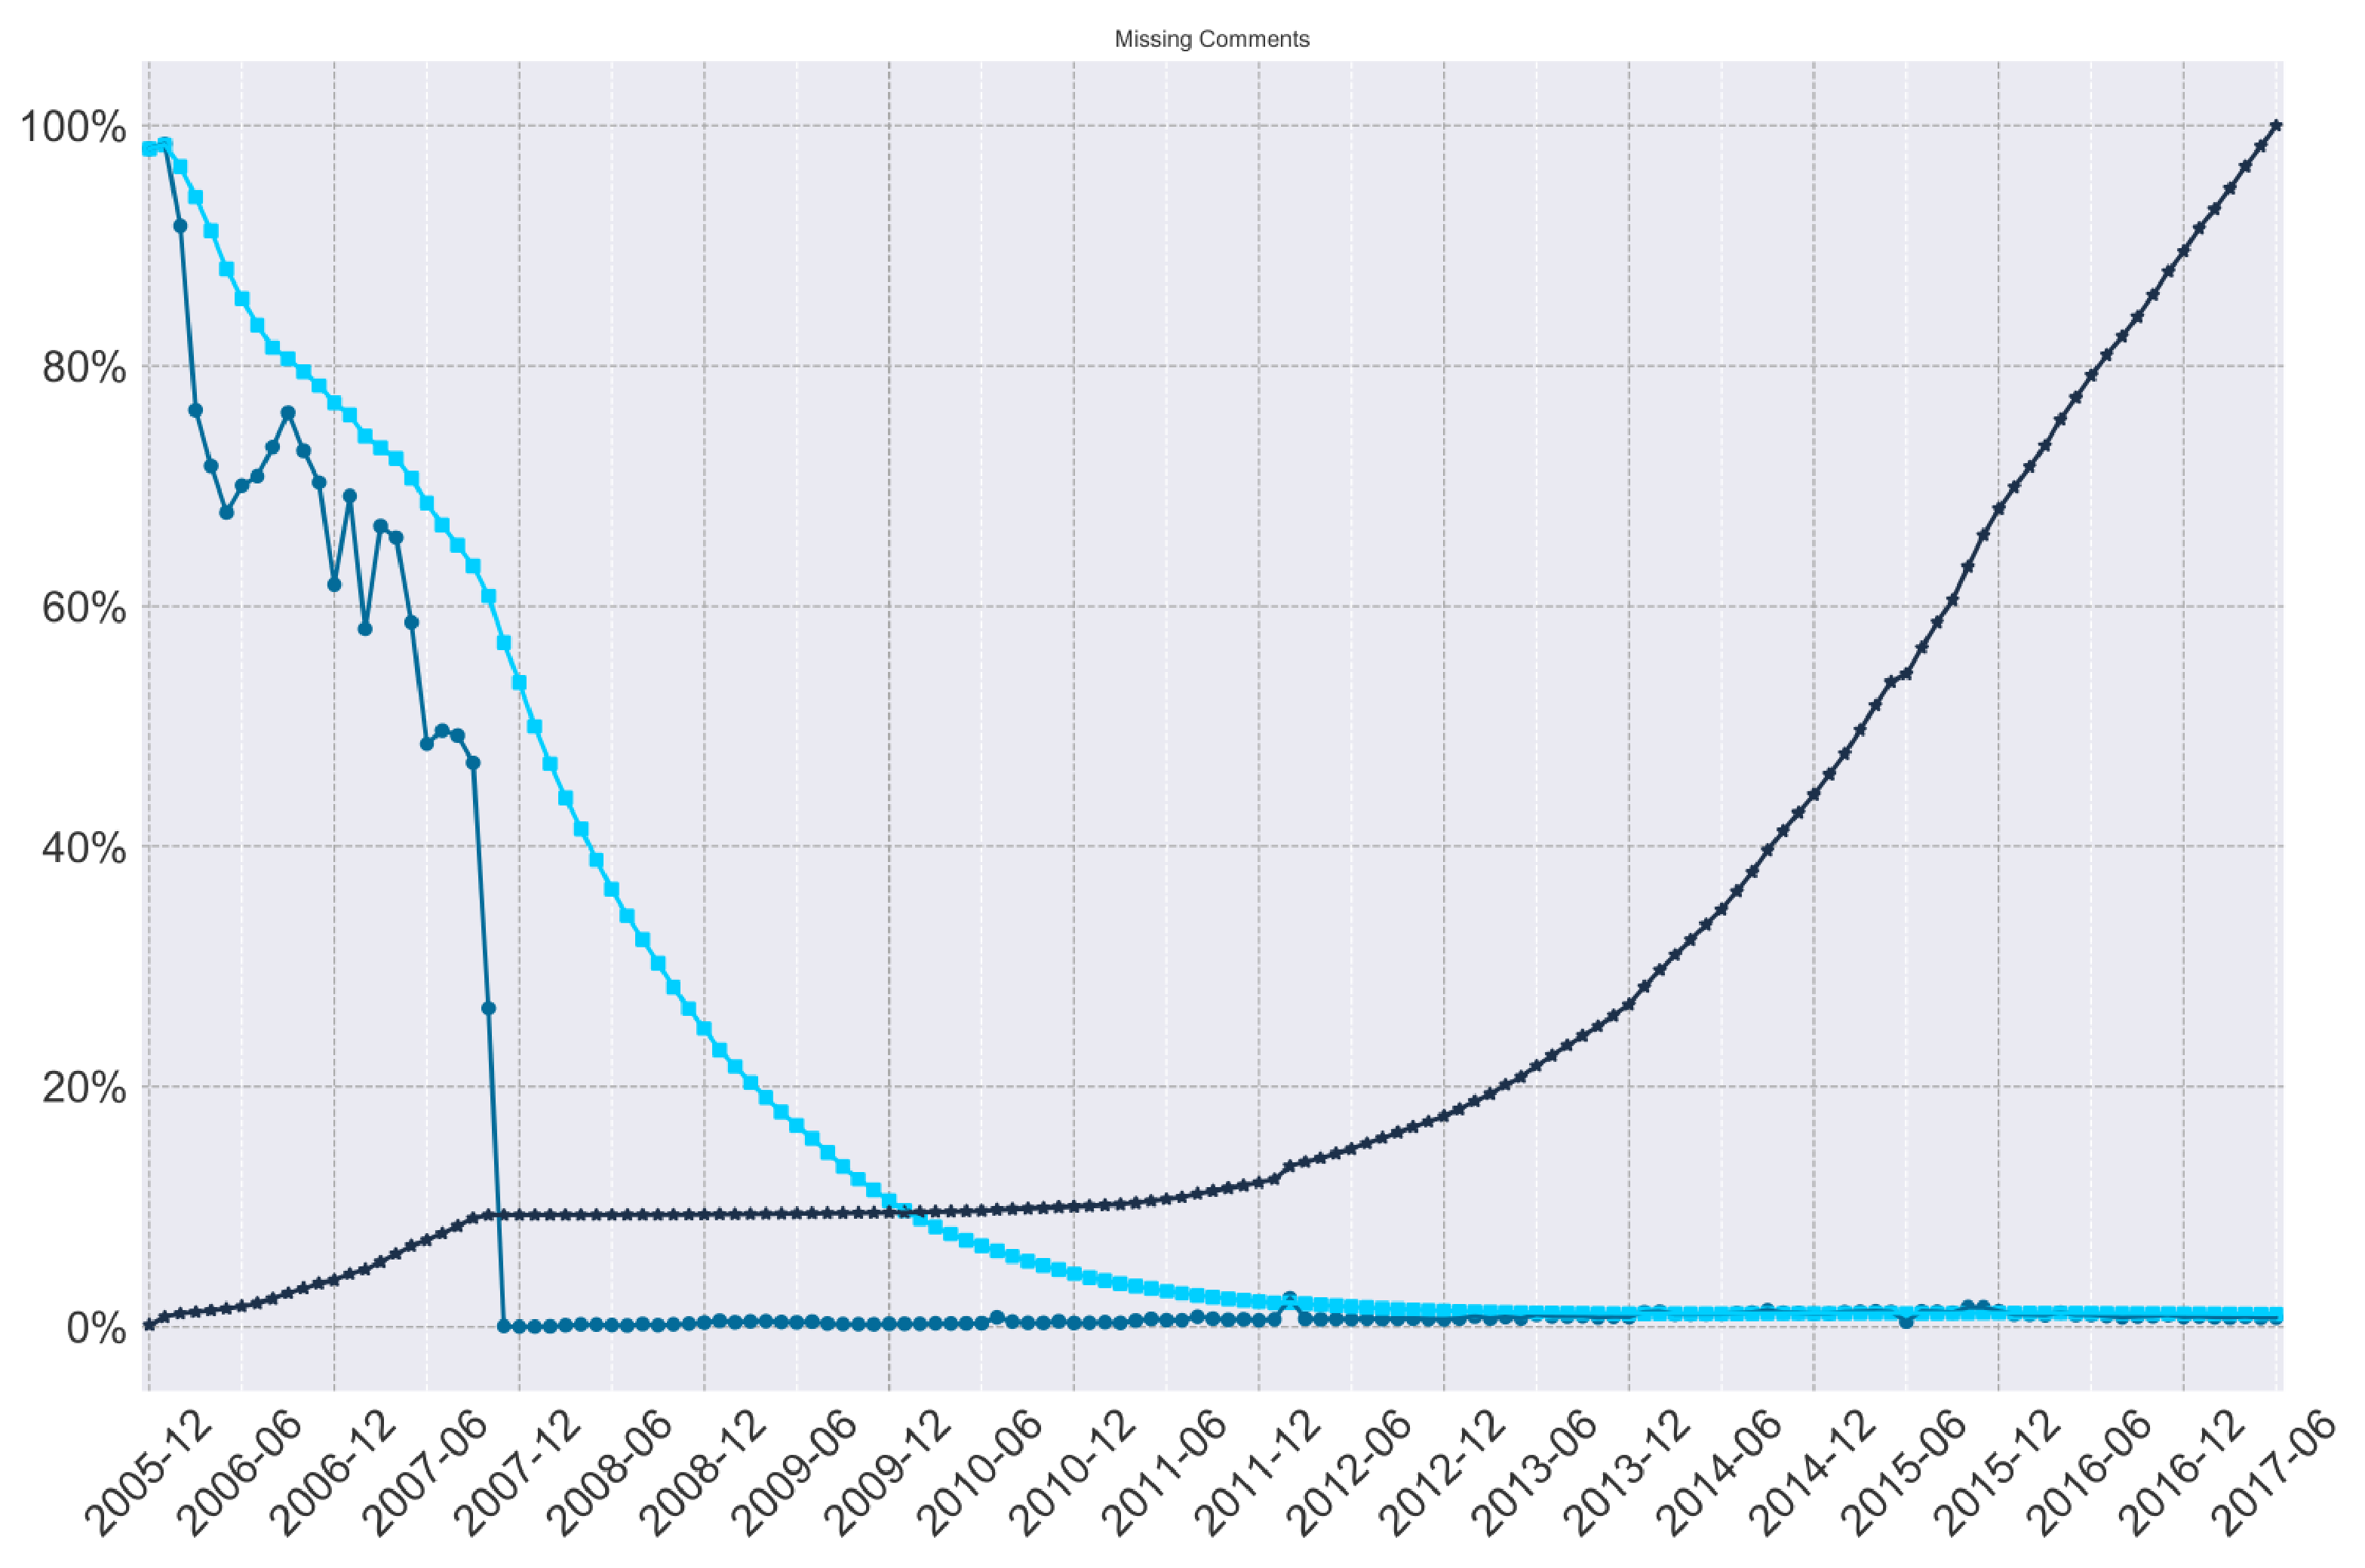
\includegraphics[width=0.8\linewidth]{./images/gaffneymatias_fig4} 

}

\caption{Anteil fehlender Kommentare. Die hellblauen Quadrate (obere
Linie) stellen den gleitenden Mittelwert fehlender Kommentare in Prozent
dar, die mittelblauen Punkte (mittlere Linie) den prozentualen Anteil
fehlender Kommentare, und die dunkelblauen Kreuze (untere Linie) die
kumlierte Gesamtzahl fehlender Kommentare \autocite{Gaffney2018}}\label{fig:gf4}
\end{figure}

In Abbildung \ref{fig:gf4} stellen die mittelblauen Punkte den Anteil
fehlender Kommentare in Prozent dar. Ab etwa April 2006 beginnt dieser
Anteil zu sinken, fällt ab etwa August 2007 stark ab und stabilisiert
sich ab etwa November 2007 im niedrigen einstelligen Bereich. Um den
Einfluss fehlender Kommentare so gering wie möglich zu halten, wurden
daher für die vorliegende Arbeit die Datensätze beginnend mit November
2007 bis einschließlich Februar 2018 ausgewertet.\\
Jason Baumgartner hat als Folge der Veröffentlichung von Gaffney und
Matias angekündigt, fehlende Kommentare und Beiträge nachträglich zu
erfassen \autocite{Baumgartner2018}.

\hypertarget{stichprobe-von-nutzern}{%
\subsubsection{Stichprobe von Nutzern}\label{stichprobe-von-nutzern}}

Nachdem der Datensatz einer zeitlichen Einschränkung unterworfen wurde,
müssen Kriterien für die Auswahl von Nutzern herangezogen werden. Dieser
Abschnitt gibt Aufschluss über die Altersverteilung von Nutzern im
Datensatz und beschreibt die Ziehung einer Stichprobe für die
Datenanalyse.

\hypertarget{altersverteilung}{%
\paragraph{Altersverteilung}\label{altersverteilung}}

Nach der zeitlichen Eingrenzung der Daten liegen für den betrachteten
Zeitraum von 124 Monaten etwa 3,6 Milliarden Kommentare vor, verfasst
von ca. 28 Millionen Nutzern. Für jeden dieser Nutzer wurde bestimmt, in
wie vielen Monaten er insgesamt im Datensatz enthalten ist; nachfolgend
wird dies als \enquote{virtuelles Alter} oder schlicht \enquote{Alter}
des Users bezeichnet.



\begin{table}

\caption{\label{tab:summary-age-tab}Zusammenfassung der Altersverteilung.}
\centering
\begin{tabular}[t]{lccccccc}
\toprule
N & arithm. Mittel & SD & Min & Q1 & Median & Q3 & Max\\
\midrule
28.029.716 & 6,67 & 12,41 & 1 & 1 & 2 & 6 & 124\\
\bottomrule
\end{tabular}
\end{table}

Tabelle \ref{tab:summary-age-tab} bietet eine Übersicht über die
Verteilung der Alterswerte. 50\% der Nutzer sind zwischen einem und
sechs Monaten auf Reddit aktiv (unteres resp. oberes Quartil), und 50\%
sind in zwei Monaten oder weniger enthalten (Median). Der arithmetische
Altersdurchschnitt liegt bei etwa sieben Monaten. Da ein User mindestens
einen Kommentar verfasst haben muss, um gezählt zu werden, liegt das
minimale Alter bei einem Monat.

\begin{figure}

{\centering \includegraphics[width=0.8\linewidth]{thesis_files/figure-latex/age-distribution-1-1} 

}

\caption{Verteilung der Alterswerte.}\label{fig:age-distribution-1}
\end{figure}

Das Histogramm in Abbildung \ref{fig:age-distribution-1} veranschaulicht
das hohe Vorkommen eher kleiner Werte. Die ALtersverteilung weist einen
sog. \enquote{Long Tail} auf: sehr viele Nutzer sind eher kurz aktiv,
während Nutzer mit eher langer Aktivität nur einen gerinen Anteil
ausmachen. Die lineare Skala des Histograms macht es schwierig, die
Werte des Long Tail sinnvoll darzustellen. Abbildung
\ref{fig:age-distribution-2} nutzt daher eine logarithmische
Darstellung.

\begin{figure}

{\centering \includegraphics[width=0.8\linewidth]{thesis_files/figure-latex/age-distribution-2-1} 

}

\caption{Verteilung der Alterswerte, logarithmische Darstellung.}\label{fig:age-distribution-2}
\end{figure}

Markant ist bei dieser Visualisierung der Ausschlag am äußersten rechten
Rand. Offenbar entfallen auf die Altersgruppe \enquote{124 Monate} noch
einmal deutlich mehr Nutzer als noch auf die vorhergehenden Gruppen. In
der Tat beträgt der Unterschied zwischen den beiden letzten
Altersgruppen 382 Nutzer Obwohl an dieser Stelle keine Erklärung für
diese Beobachtung geliefert werden kann, ist es denkbar, dass es einen
\enquote{harten Kern} von Usern gibt, die Reddit seit langer Zeit,
möglicherweise sogar von Anfang an nutzen, und regelmäßig aktiv sind.

\hypertarget{kriterien-fur-die-stichprobe}{%
\paragraph{Kriterien für die
Stichprobe}\label{kriterien-fur-die-stichprobe}}

Um Nutzer für die weitere Datenanalyse auszuwählen, wurden zwei
Kriterien festgelegt. Zum einen sollte ein Nutzer über einen ausreichend
langen Zeitraum hinweg aktiv sein. Damit wird sichergestellt, dass
zeitliche Verläufe keine Lücken aufweisen und genügend Daten vorliegen,
um Trends zu identifizieren. Zum anderen sollte der User ein Mindestmaß
an Interaktionen pro Monat hervorbringen. Da diese Arbeit
Interaktionsgraphen analysiert, sollten di

Für die Analyse treffen wir eine Zufallsauswahl aus den ältesten 1000
Usern. Dadurch stellen wir sicher, dass wir User über einen genügend
langen Zeitraum beobachten können. Das folgende Histogramm zeigt die
Verteilung dieses Ausschnitts aus dem Long Tail.

\hypertarget{topic-modelling}{%
\subsubsection{Topic-Modelling}\label{topic-modelling}}

Für die Berechnung des Topic-Modells wurden für eine Auswahl an
Subreddits die Titel von 50 Beiträgen aus der \emph{Top}-Kategorie

Für jeden Kommentar im Datensatz wurde festgehalten, in welchem
Subreddit er erstellt wurde. Kommentare, deren Schlüssel \texttt{author}
den Wert \texttt{{[}deleted{]}} enthielten, wurden dabei übersprungen;
Reddit nutzt diesen Wert, um gelöschte Inhalte zu kennzeichnen.

\hypertarget{ego-netzwerke-und-soziale-netzwerkanalyse}{%
\subsubsection{Ego-Netzwerke und soziale
Netzwerkanalyse}\label{ego-netzwerke-und-soziale-netzwerkanalyse}}

\hypertarget{ergebnisse}{%
\subsection{Ergebnisse}\label{ergebnisse}}

\hypertarget{das-alter-von-usern}{%
\subsubsection{Das Alter von Usern}\label{das-alter-von-usern}}

In den vorangehenden Kapiteln wurde erläutert, welche Daten gesammelt
wurden und wie eine erste Vorauswahl getroffen wurde. Die detaillierte
Analyse soll Gegenstand dieses Kapitels sein.

\hypertarget{virtage}{%
\paragraph{Virtuelles Alter}\label{virtage}}

Nach der Vorauswahl der Daten ergibt sich ein Analysezeitraum von 124
Monaten. Da nicht alle Nutzer über diesen gesamten Zeitraum hinweg aktiv
gewesen sein werden, ist eine weitere Auswahl nöitg. Zudem ist es
denkbar, dass ein Teil der Nutzer nach nur wenigen Monaten die Plattform
wieder verlassen hat.

Zur Bestimmung des virtuellen \enquote{Alters} der Nutzer, also wie
lange sie sich aktiv an Reddit-Communities beteiligen, wurde für jeden
Monat erfasst, in welchen Subreddits sie aktiv sind und wieviele
Kommentare sie dort verfassen. Diese monatlichen Daten wurden dann über
den gesamten Zeitraum aggregiert, sodass am Ende für jeden Nutzer
ersichtlich war, in wie vielen monatlichen Zusammenfassungen er
auftaucht, sprich: wie viele Monate er sich aktiv beteiligt hat.

\textbf{PLACEHOLDER USER AGESPLACEHOLDER USER AGES}

Wie in Abbildung\textasciitilde{}\ref{fig:virt_alter} ersichtlich liegen
75\% der Daten unterhalb des Mittelwerts, viele User sind also weniger
als 6 Monate auf Reddit aktiv. Um sinnvolle Aussagen über die zeitliche
Entwicklung treffen zu können, werden nur Nutzer betrachtet, die
mindestens 6 Monate aktiv waren. Damit verbleiben
7\textsubscript{047}535 Nutzer im Datensatz, was etwa 25\% der
Gesamtzahl entspricht.
Abbildung\textasciitilde{}\ref{fig:virt_alter_geschnitten} zeigt die
Verteilung für diesen neuen Datensatz.

Für diese Nutzer werden die Subreddits erfasst, in denen sie aktiv sind.
Über die Reddit-API werden zu jedem dieser Subreddits 50 Beiträge aus
der \textit{Top}-Kategorie abgerufen, welche die höchstbewerteten Posts
dieser Community auflistet, unabhängig vom Erstellungsdatum des
Beitrags. Diese Top-Beiträge dienen im weiteren Verlauf dazu, ein
Subreddit inhaltlich zu charakterisieren; ihre Titel werden einer
Topic-Analyse unterzogen.

\textbf{PLACEHOLDER USER AGES}

\begin{table}[h]
    \centering
    \begin{tabular}{lccccc}
        \toprule
        & N & Mittel & Median & Min & Max \\
        \midrule
        voller Datensatz & 28~029~500 & 6,665$\pm$12,407 & 2 & 1 & 124 \\
        mindestens 6 Monate aktiv & 7~047~535 & 21,593$\pm$17,634 & 15 & 6 & 124 \\
        \bottomrule
    \end{tabular}
    \caption{Altersverteilungen}%
    \label{tab:altersverteilungen}
\end{table}

Beim Abrufen der insgesamt 419\textasciitilde{}616 Subreddits antwortete
die Reddit-API in XY Fällen mit \glqq{}404 Not Found\grqq{}, und in XY
Fällen mit \glqq{}403 Forbidden\grqq{}. Die genaue Ursache dieser Fehler
kann nicht bestimmt werden, aber 404 lässt vermuten, dass das Subreddit
gelöscht wurde, und 403 deutet auf eine zugangsbeschränkte Community
hin, die nicht frei einsehbar ist.

Wegen eines Programmierfehlers wurden zu 499 Usern nicht die Subreddits
abgerufen, in die sie gepostet hatten. Eine nachträgliche Analyse ergab,
dass diese Nutzer im Mittel einen Monat aktiv waren und 1,17 Kommentare
verfassten. Aufgrund dieser geringen Aktivität wurde keine Nacherfassung
der Subreddits durchgeführt.

\hypertarget{verteilung-von-topics}{%
\subsubsection{Verteilung von Topics}\label{verteilung-von-topics}}

\hypertarget{fallstudie}{%
\subsubsection{Fallstudie}\label{fallstudie}}

\cleardoublepage

\hypertarget{diskussion}{%
\section{Diskussion}\label{diskussion}}

\cleardoublepage

\hypertarget{zusammenfassung-und-ausblick}{%
\section{Zusammenfassung und
Ausblick}\label{zusammenfassung-und-ausblick}}

\printbibliography


\end{document}
